\section{Electronics}



The photomultiplier tubes are the XP4500B from Photonis. They are powered in positive polarity by CAEN SY4527. The CAEN boards are controlled by slow control software.

The high voltage cable is connected to the inside of the LTCC through a patch panels with hermetical connectors, also used for the PMT outputs.

One of the PMT output is connected directly to Flash ADC boards built at Jefferson Lab (FADC250)(REF). The other output is connected to CAEN v1190 TDC modules.

In \F{fadc} a digitized signal from the FADC module is shown. The FADC sampling frequency is $250 MHz$ and the signal is typically contained in 3-4
samples.

\begin{figure}
	\centering
	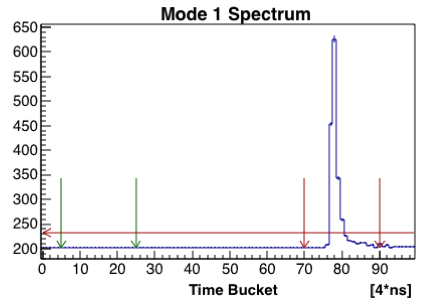
\includegraphics[width=0.95\columnwidth,keepaspectratio]{img/fadc.png}
	\caption{The FADC250 digitized output from one of the LTCC channel self triggering on the single photo-electron signal. The samples are 4 ns apart, for a total of 100 samples. }
	\label{fig:fadc}
\end{figure}


The electronic scheme is shown in \F{electronicScheme}.

\begin{figure}
	\centering
	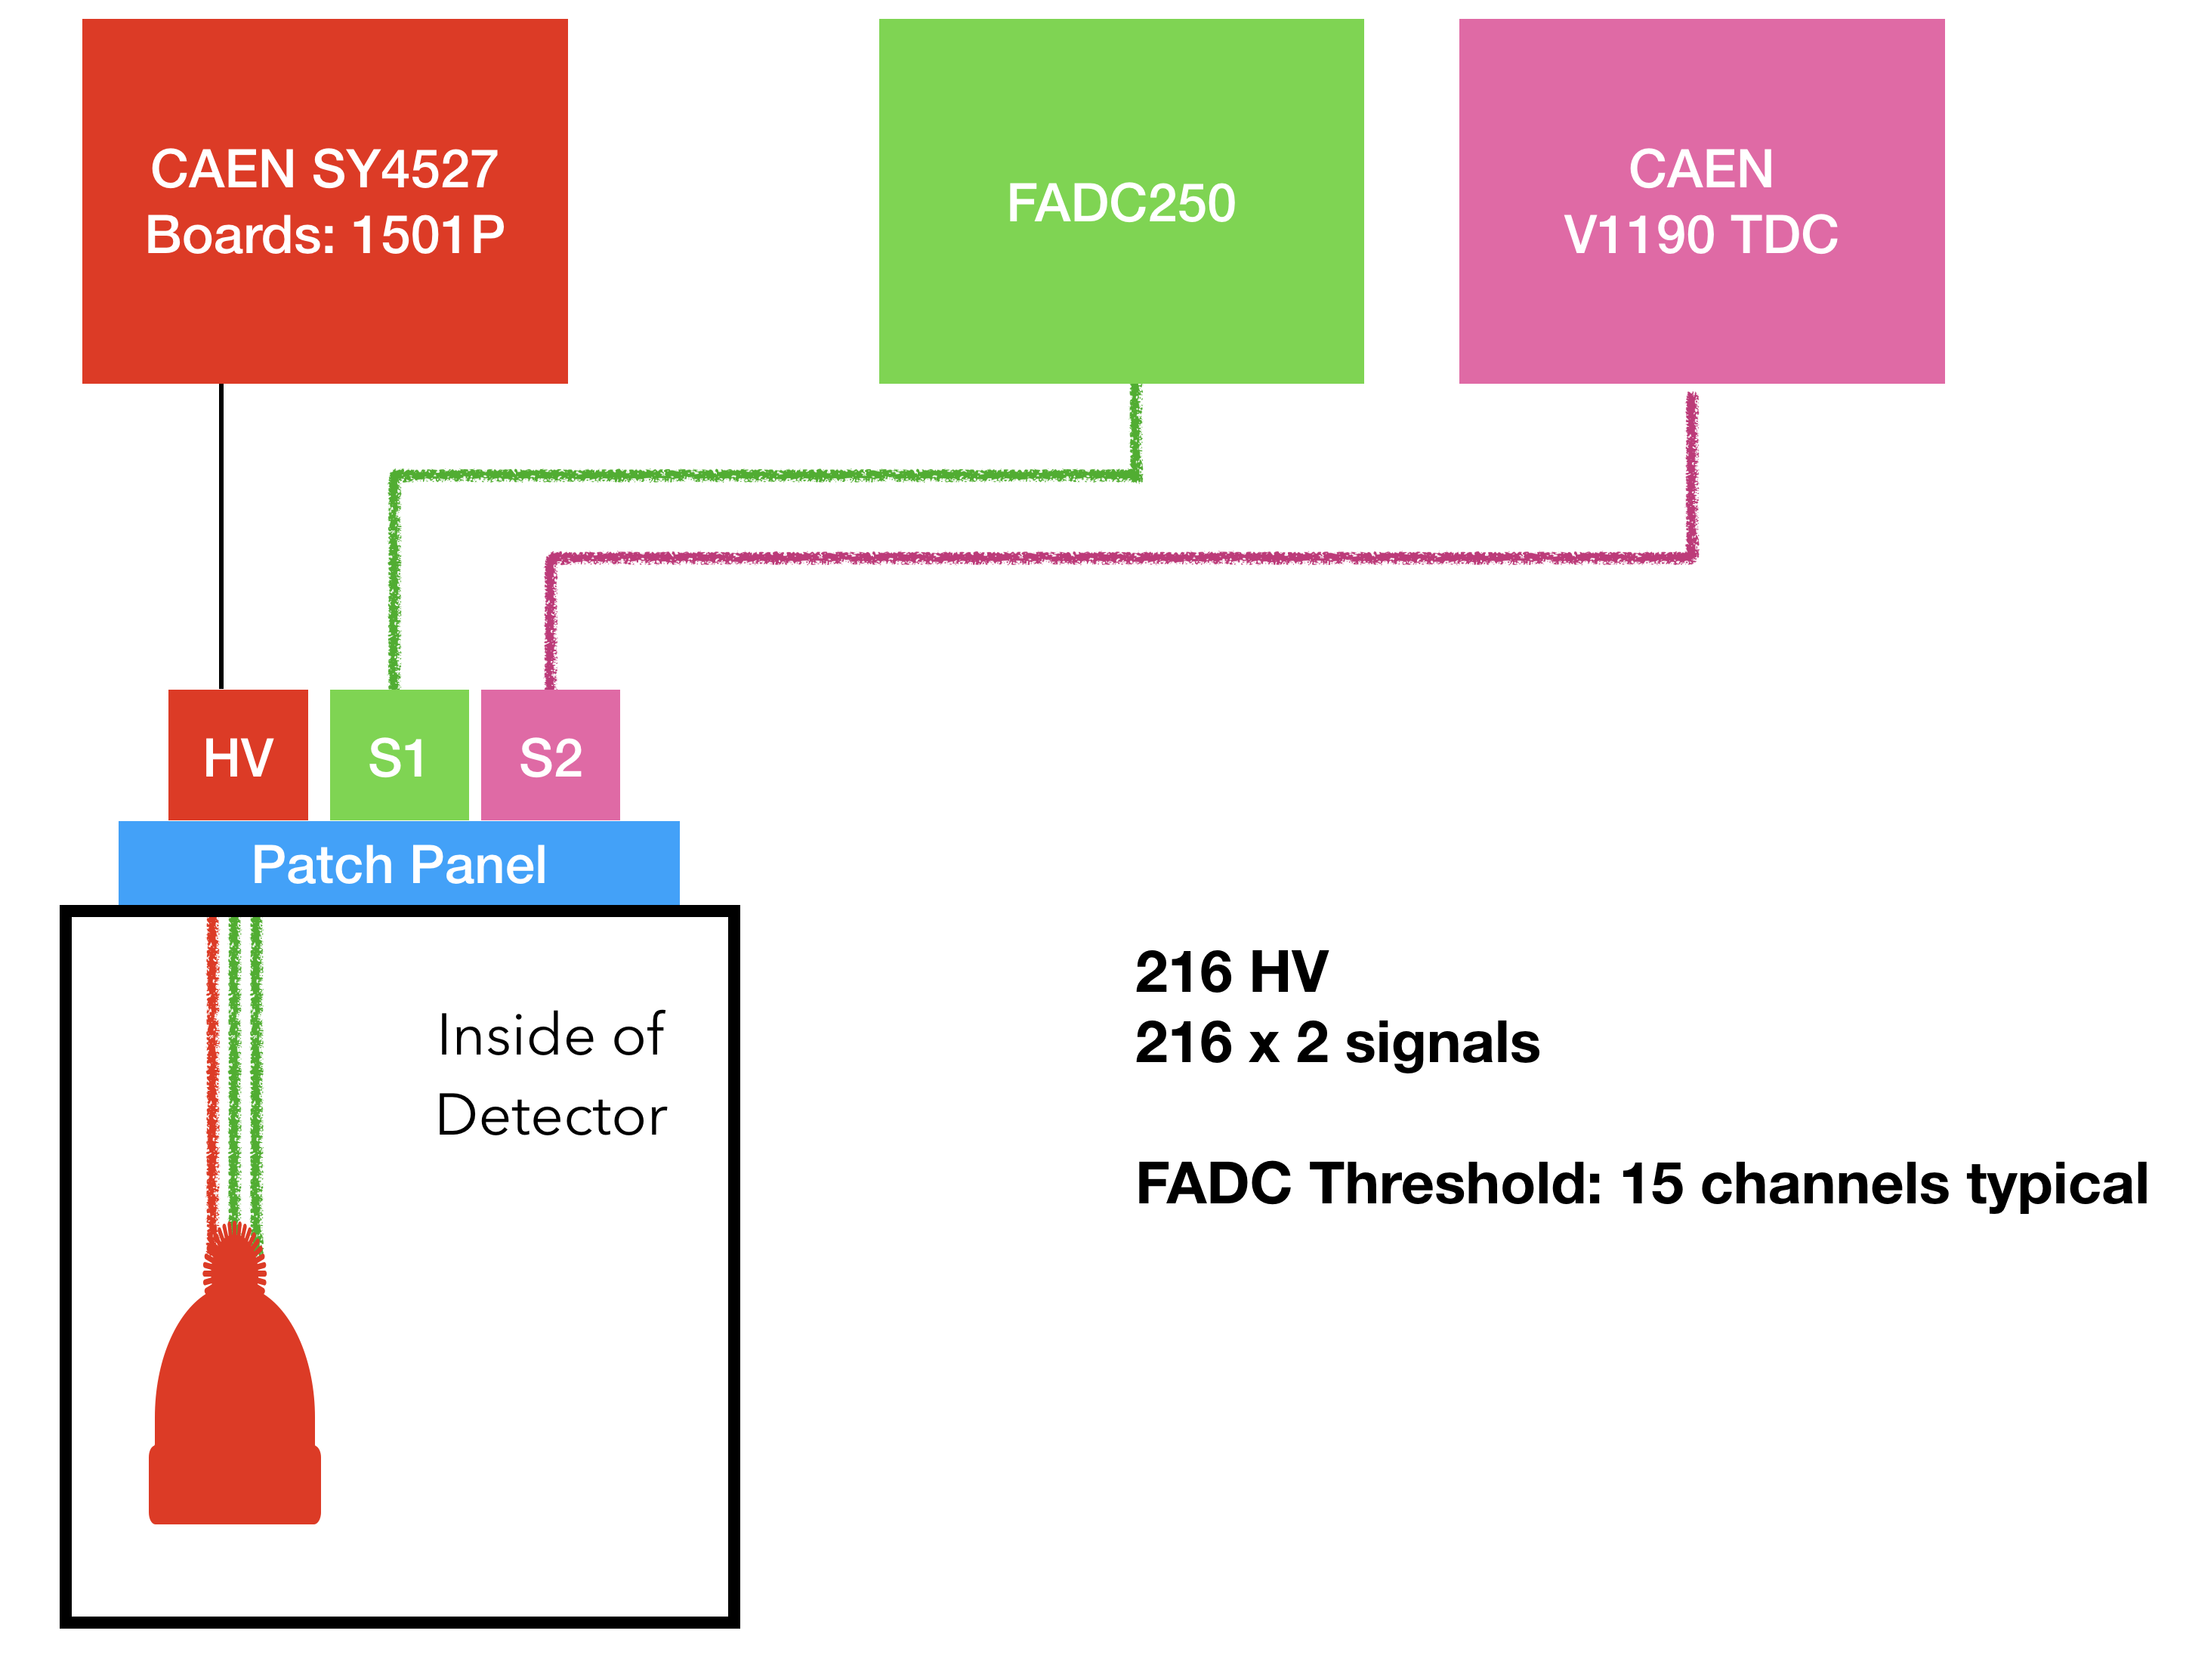
\includegraphics[width=0.95\columnwidth,keepaspectratio]{img/electronicScheme.png}
	\caption{The electronic scheme of the LTCC.}
	\label{fig:electronicScheme}
\end{figure}
